\scanpage{34}

2. \uline{Accouplements définis par une biextension}.

2.1. Soit $n$ un entier $>0$, et supposons qu'on a
\[
(2.1.1)\qquad nP=P.
\]
Considérons alors l'homomorphisme composé
\figure{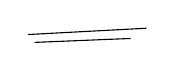
\begin{tikzpicture}\draw (0,0)--(1.5,.08);\draw (.08,-.1)--(1.3,-.05);\end{tikzpicture}}

(2.1.2)
\diagram{\begin{tikzcd}[ampersand replacement=\&, column sep=large]
\operatorname{Biext}^{\inserted{1}}(P,Q;G) \arrow[r] \arrow[rr,bend left=20,"\phi^n"] \& \operatorname{Biext}^{\inserted{1}}(P,{}_nQ;G) \arrow[r,"\sim"] \& \operatorname{Hom}({}_nP\otimes{}_nQ;G)
\end{tikzcd}},

où la première flèche est la restriction à $(P,{}_nQ)$, et la deuxième est l'isomorphisme (1.3.6). Il permet, à tout élément \figure{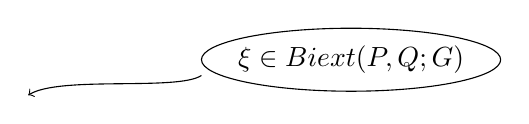
\begin{tikzpicture}[baseline=(x.base)]\node(x){$\xi\in\operatorname{Biext}(P,Q;G)$};\draw(0,0)ellipse(1.9 and .4);\draw[->](-1.9,-.2)..controls(-2.2,-.4)and(-3.7,-.2)..(-4.1,-.45);\end{tikzpicture}},

(2.1.3)

à fortiori à toute biextension \inserted{\figure{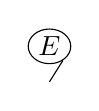
\begin{tikzpicture}[baseline=(e.base)]\node(e){$E$};\draw(0,0)ellipse(.27 and .22);\draw(.17,-.18)--(0,-.45);\end{tikzpicture}}} de $(P,Q)$ par $G$, de faire correspondre un\deleted{e \unsure{forme homomorphisme}} accouplement bilinéaire
\margin{\figure{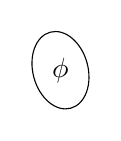
\begin{tikzpicture}\node at(0,0){$\phi$};\draw[rotate=15](0,0)ellipse(.35 and .5);\end{tikzpicture}}}
\[
(2.1.4)\qquad\phi_\xi\text{ ou }\phi^n_\xi:{}_nP\times{}_nQ\longrightarrow G,
\]
qu'on appelle l'accouplement \uline{associé à} $\xi$ (ou à la biextension $E$).

2.2. Soit \deleted{\unsure{n}} $n'$ un multiple de $n$,
\[
n'=mn,
\]
et supposons qu'on ait la relation (plus forte que (2.1.1))
\[
(2.2.1)\qquad n'P=P\quad\text{i.e.}\quad mnP=P,
\]
d'où comme en (2.1.4), pour toute $\xi\in\operatorname{Biext}(P,Q;G)$, un\deleted{e} accouplement
\[
\phi^{n'}_\xi:{}_{n'}P\times{}_{n'}Q\longrightarrow G.
\]
\deleted{Les relations entre cet accouplement et}\inserted{Il est lié à} l'accouplement $\phi^n_\xi$ \deleted{est donné} par la commutativité du diagramme suivant (\deleted{qu'on laisse au lecteur le soin d'établir)}\inserted{cf. 2.3 ci-dessous pour une démonstration)}:

(2.2.2)
\diagram{\begin{tikzcd}[ampersand replacement=\&, column sep=small,row sep=large]
{}_{n'}P \arrow[d,"m"'] \& \times \& {}_{n'\deleted{\unsure{n}}}Q\deleted{\unsure{Q}} \arrow[d,"m"] \arrow[rr,"\phi^{n'}_\xi"] \& \& {}_{n'}G \arrow[d,"m"]\\
\deleted{\unsure{P}}{}_nP \& \deleted{\unsure{\times}}\times \& {}_nQ \arrow[rr,"\phi^n_\xi"] \& \& {}_nG
\end{tikzcd}},
\inserted{où les flèches verticales sont induites par la multiplication par $m=n'/n$.}

Notons maintenant que moyennant (2.1.1), on peut prendre pour $n'$ n'importe quelle puissance de $n$. En particulier, soit \figure{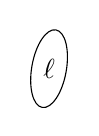
\begin{tikzpicture}[baseline=(l.base)]\node(l){$\ell$};\draw[rotate=-10](0,0)ellipse(.22 and .5);\end{tikzpicture}} un nombre premier, et supposons que\deleted{\unsure{e}} l'on ait
\margin{\figure{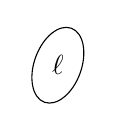
\begin{tikzpicture}\node at(0,0){$\ell$};\draw[rotate=-20](0,0)ellipse(.3 and .5);\end{tikzpicture}}}
\[
(2.2.3)\qquad\figure{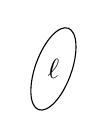
\begin{tikzpicture}[baseline=(l.base)]\node(l){$\ell$};\draw[rotate=-20](0,0)ellipse(.23 and .55);\end{tikzpicture}} P=P,
\]
et considérons le système des accouplements
\margin{33}
